\begin{figure*}[t!]
\centering
%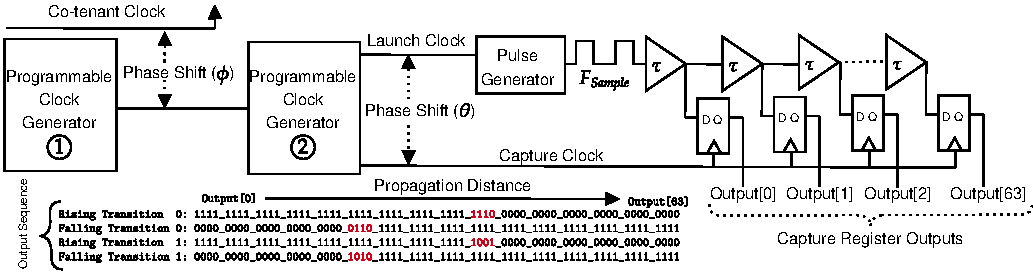
\includegraphics[width=0.9\linewidth]{img/dl-schema.pdf}
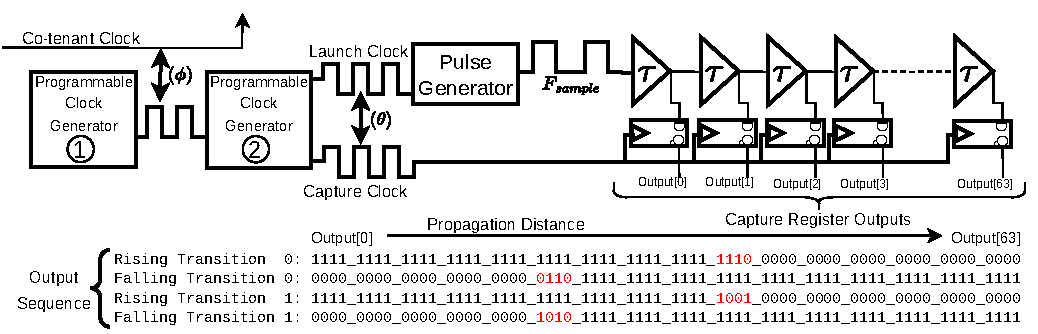
\includegraphics[width=0.9\linewidth]{img/TDC_MT.pdf}
\vspace{-10px}
\caption{\name Time-To-Digital Converter Architecture: A pulse generator produces falling and rising transitions that propagate through delay line elements. %The propagation characteristics are studied in this paper. 
Output capture registers record the transitions based on the capture clock. PDN voltage fluctuations affect the propagation speed and cause variations in the transition point (\textcolor{red}{red}).}
\label{fig:dl-schema}
%\cd{TODO - cleanup angular lines. Make up boxes smaller. Make Output Sequence horizontal.}
\vspace{-10px}
\end{figure*}